% Конкретные численные значения, которые использовались (входные данные)

Для проведения экспериментов использовалась модель с следующими численными значениями:
\begin{center}
  $l = 1, n = 5, m = 4, k = 3$
\end{center}

Для этих числовых значений составлены матрицы:
\begin{center}
  $
  T = 
  \begin{pmatrix}
      1 &   0 &   0 & 0   \\
    0.5 & 0.5 &   0 & 0   \\
      0 & 0.5 & 0.5 & 0   \\
      0 &   0 & 0.5 & 0.5 \\
      0 &   0 &   0 & 1 
  \end{pmatrix}
  $
\end{center}

\begin{center}
  $
  D = 
  \begin{pmatrix}
    0 & 0 & 0 & 0   \\
    0 & 0 & 1 & 1   \\
    0 & 0 & 0 & 0   \\
    0 & 0 & 0 & 0 
  \end{pmatrix}
  $
\end{center}

\begin{center}
  $
  P = 
  \begin{pmatrix}
    1 & 1 & 1 & 1 & 1   \\
    1 & 1 & 1 & 1 & 1   \\
    1 & 1 & 1 & 1 & 1   \\
    1 & 1 & 1 & 1 & 1   \\
    1 & 1 & 1 & 1 & 1 
  \end{pmatrix}
  $
\end{center}

\begin{center}
  $
  E = \begin{pmatrix}
    1 & 0 & 0 & 0 & 0
  \end{pmatrix}
  $
\end{center}

% Рисунок (граф со стрелками и связями) модели, которую обсчитываем

Графическое представление в виде графа построенного в соответствии с описанными выше исходными данными модели изображено на рисунке \ref{fig:graph}.

\begin{figure}[H]
  \centering
  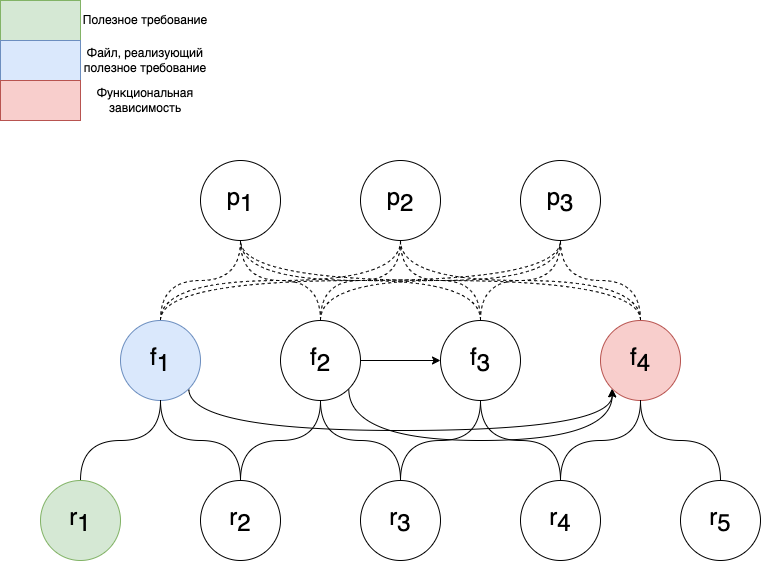
\includegraphics[width=0.8\textwidth]{graph}
  \caption{Графическое предствление в виде графа}
  \label{fig:graph}
\end{figure}

% Информация из принта модели с указанием общего числа параметров модели и ее ограничений

Результирующая математическая модель включает $54$ ограничения и $32$ параметра. Из них $12$ являются искомыми значениями, а $20$ дополнительными параметрами.

% Таблица с применением решателей для решения моей сформированной модели

% Для каждого из используемого решателей привести информацию о вычисленном значении целевой функции 
